\begin{savequote}[75mm] 
If I have seen further it is by standing on the shoulders of giants
\qauthor{Isaac Newton} 
\end{savequote}

\chapter{Introduction}

\newthought{Bioinformatics is in its very nature multi--disciplinary}: biotechnology methods are used to capture the data, mathematical and statistical models are necessary to make sense of it; and software/hardware it is necessary to process all the information and everything should be seen under the prisma of the existing biological knowledge.

Techniques and methods trying to uncover the logic behind cellular proceses are in constant development. The success of such methods is usually related to the ability of isolating a particular state/measurement of the organic material (e.g. level of expression of a single protein, number of mutations of a gene in a population, etc.). However,  cellular functions of a higher level and organism's processes can only be study with a more holistic approach.

Integrating information from different experiments in context with the current knowledge-base is one of the most recurrent duties that researchers have to accomplish, this task however takes another dimension when the goal is aimed to a generic scope, and the strategy to connect related data sets should work in similar scenarios.

The challenges of integrate data in a more generic scope go from technical (e.g. incompatibilities of the storage systems) to structural (e.g. two datasets can refer to the same entity using different identifiers), but in overall the major challenge is to not lose the meaning on the connection (e.g. linking proteins and genes and knowing what is their relationship).

Integration of data usually refers to connecting data in low level, by means of storing aggregated information from several sources or by saving links to where the source is. However it is also possible to integrate on a higher level, where information is not saved and the aggregates are built on the fly and visualised in order to provide a wider view.

This project explores both, Integration and visualisation of information in bioinformatics; the rest of this introduction presents the state of the art and base technologies in both fields. Chapter 2 presents the efforts executed during this doctorate that contribute to the ways data is integrated in bioinformatics projects. Chapter 3 describes our inputs to the visualisation of data in bioinformatic, focusing in particular in a web tool for the visualisation of protein-protein interactions. The final chapter contains the conclusions of the project.


\section{Integration of information}
\subsection{State of the art}
The latest version of the Nucleic Acids Research Database Issue added another 58 databases to the online collection hold by the journal, which then reached the number of 1552 databases \cite{FER2014}. This collection is far from including every single database, but it is  a good reflection of the amount of available resources.
The approaches to integrate data from all those sources are themselves heterogenous and they focused on different types of integration, from simply linking resources; to development of complex structures of aggregated information. In \cite{GOB2008} the authors categorise the different techniques used to integrate data in bioinformatics into 8 approaches, and then this categories were reorganised in \cite{ZHA2011b} into:
\begin{description}
\item[Data warehousing:] 			A centralised repository were the information from different sources is copied and processed to be kept  in a single place. providing a single access point to their data. However the preprocessing of the data is usually a complex process and the posterior additions or editions might require a lot of work.
\item[Federated databasing:] 		Multiple sources agree to follow a similar structure in order to allow a standard query over several instances. By dealing with smaller datasets than the data warehousing approach the complexity of post-processing is simplified, however it requires that the providers deal with the extra work of maintaining their data as the federated database agreement stablishes.
\item[Service oriente integration:] 	Definition of a protocol for requests and responses to obtain data or execute services. The 2 standards widely used are SOAP (Simple Object Access Protocol) services and REST (REpresentational State Transfer) services, where the latter is getting momentum because of its simplicity. However this also requires big commitment from providers about creating and maintaining the services, and also increasing and maintaining the specifications for the different domains.
\item[Semantic integration:] 		Structures the data using semantic web standards(e.g. RDF, OWL) in order to make it ``machine-readable'' and be able to deduce meaningful associations. The conversion of the data into RDF files might not be a trivial work, and it has similar problems to the one mentioned above because it maintains copies of the information in a separate format. 
\item[Wiki-based integration:] 		Cooperative effort where the community inputs information in a open and unstructured way, which can reach a highly reliable status as has been shown by the wikipedia case, but is completely dependent on the adoption of the community, and also given the unstructured nature of the data is hard to manipulate for automatic analysis.
\end{description}

We now present some of the most representative projects that have attempted to integrate data and offer a solution for this need in the bioinformatics field, by using one or more of the mentioned approaches. 

\subsubsection{Sequence Retrieval System}
The Sequence Retrieval System, better known in bioinformatics as SRS, was probably the most successful project before the introduction of Next Generation Sequencing (NGS) technologies, originally aimed at facilitating access to biological sequences databases \cite{ETZ1996}, it grew to became an integration system of both data retrieval and applications fro data analysis.

SRS was developed following an object-oriented design with the strategy of taking advantage of raw text files, that were the \emph{de-facto} standard on molecular biology analysis. By dealing only with text files, SRS was getting faster retrieving speed and saving storage space, mainly because data was neither store nor parsed, only indexed \cite{ZDO2002}.

The obtained indexes were there linked via meta-data, offering the user access to the original source plus links to any conceptually related database; all of it presented on a web-based interface, the automatically created interface for different sources and applications can be complicated for beginners, however SRS provide ways to create customised interfaces.

Probably the most important instance of SRS was the one installed at the European Bioinformatics Institute (EBI), which used to give access to the major databases produced and maintained at the EBI. However by December 2013 the service was decommissioned as the service was considered redundant with the efforts to maintain multiple web services. Currently SRS technology is now property of Instem\textsuperscript{TM} and a list of available servers can be seen at http://bioblog.instem.com/download/srs-parser-and-software-downloads/public-srs-installations/


%\section{Current Projects for Data Integration in Bioinformatics}
\subsubsection{BioWarehouse}
BioWarehouse is an open source toolkit to create data warehouses using MySQL or Oracle \cite{LEE2006}. The motivation behind this project is to provide  a single access point that supports Standard Query Language (SQL) running on a high performance environment.
This projects follows the data warehousing approach to integrate data, however the authors argue that it can be use as a part on a federated system and therefore, it doesn't aim to replace existing distributed system but o to complement them.

The development efforts were focused on the creation of a relational data model that supports the information from several biologic entities. Figure ~\ref{fig:biowarehouse} shows the main datatypes that are defined in the BioWarehouse scheme including, Taxon, BioSource, Nucleic Acid, Gene, Protein, Feature, Reaction, Chemical and Pathway. It was the objective of the creators that such model evolves including other entities, but at the same time keeping the model as simple as possible.

\begin{figure}  
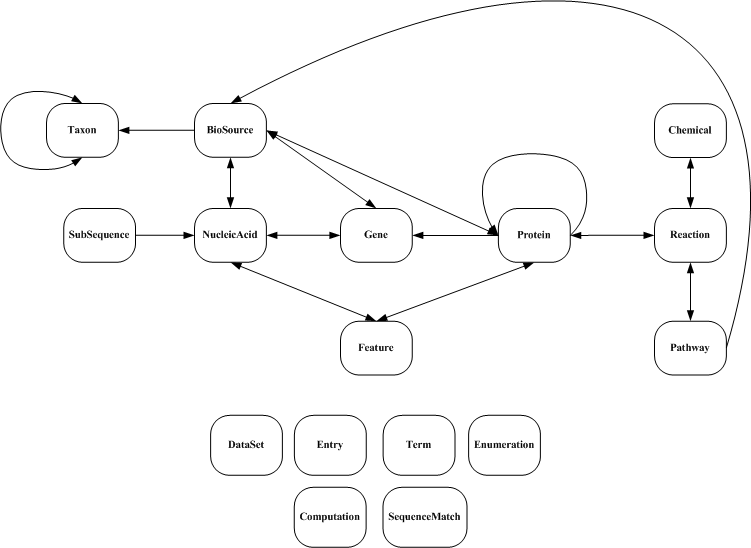
\includegraphics[width=4in]{figures/biowarehouse.png}
\caption[Original BioWarehouse schema.]{The main datatypes in the BioWarehouse schema, and the relationships between them.
\label{fig:biowarehouse}}
\end{figure}

The package that composes BioWarehouse includes a set of loaders implemented in java and C++, that allows to automatise the loading of data from several popular sources. 

An instance of BioWarehouse called Publichouse is available online https://publichouse.ai.sri.com/phpmyadmin/ (last checked December 2014) and provides access to compiled data from: NCBI Taxonomy, Enzyme, MetaCyc Chemical Compound Ontology, MultiFun Gene Ontology, MetaCyc Pathway Ontology, BioCyc, Swiss-Prot and TrEMBL.

The most recent contribution reported in their website is from August 2010 installing the web based interface for mysql databases called myphpadmin. This puts in evidence the little development that the project have have in the last 4 years. A similar situation have been observed in projects that follow the same warehousing strategy in bioinformatics. Most of them published around the same period of time but inactive in recent years, or with broken links to the tool, for example, Atlas \cite{SHA2005} published in 2005, LCB\cite{AME2006} published in 2006 and M-Chips \cite{FEL2002} from 2002. From our research the only active project on infrastructure of data warehousing for biological data is BioDWH, which is described below.

\subsubsection{BioDWH}
The data warehouse for life science data Integration known as BioDWH is a project developed at  the Bielefeld university. BioDWH is a Java based project that developed an object-relational mapping using the library Hibernate to connect to the most common relational database management systems RDBMS (e.g. MySQL, Oracle, PostgreSQL) in order to create a centralised repository that integrates information from various biological databases \cite{TOP2008}.

BioDWH main objective is to increase customisation of the data warehouse concept improving performance, scalability and having quality data up to date. As part of the project they have included some parsers to extract information from well-known available resources (e.g. UniProt, KEGG, OMIM, etc.). Figure ~\ref{fig:biodwh} presents the extensions to a general data warehouse design done in this project in order to define an architecture oriented to life sciences data.

\begin{figure}  
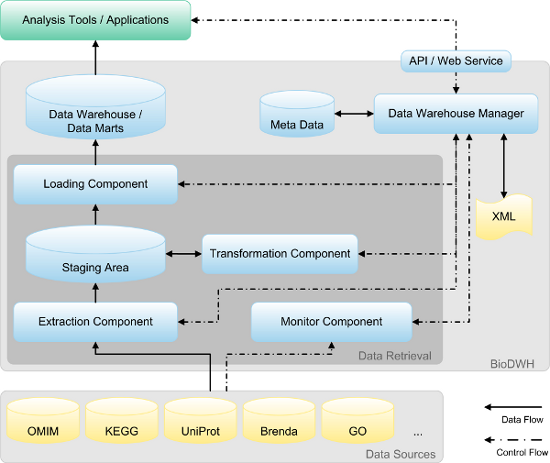
\includegraphics[width=4in]{figures/dwh_architecture.png}
\caption[BioDWH System Architecture.]{BioDWH System Architecture.
\label{fig:biodwh}}
\end{figure}

It is important to highlight the inclusion of a monitor system that keeps track on the need of updates from the different sources. Instead of direct access to the RDBMS, BioDWH provides an API that can be queried remotely, and a Graphical User Interface, that enables the configuration of the different components including monitors and parser besides the queuing and displaying of content.

Two projects have been reported in he literature to be using BioDWH: DAWIS-M.D. and VANESA. DAWIS-M.D. is oriented to metabolic data and integrates 11 different databases: BRENDA, EMBL, HPRD, KEGG, OMIM, SCOP, Transfac, Transpath, ENZYME, GO and UniProt. \cite{HIP2010}. VANESA uses DAWIS-M.D. in order to access important information for the modelling of biological processes and systems as biological networks\cite{BRI2014}.

\subsubsection{BioMart}
BioMart started by using the same principle of data warehousing that BioWarehouse, BioDWH and other projects of data warehouse in life science have follow: ``\emph{to create one universal software system for biological data management and empower biologists with the ability to create complex, customised datasets}'' \cite{KAS2011}.

With this object in mind BioMart have grown from an extension to the Ensembl website for data mining, to become an international effort for the integration of biological data. This has been achieve by first defining a general software infrastructure for further customisation, and then extending this architecture in order to support multi-database repositories as a data federation system, where all the entities use a predefined relational schema, that is generic enough to support any kind of data.

\begin{figure}  
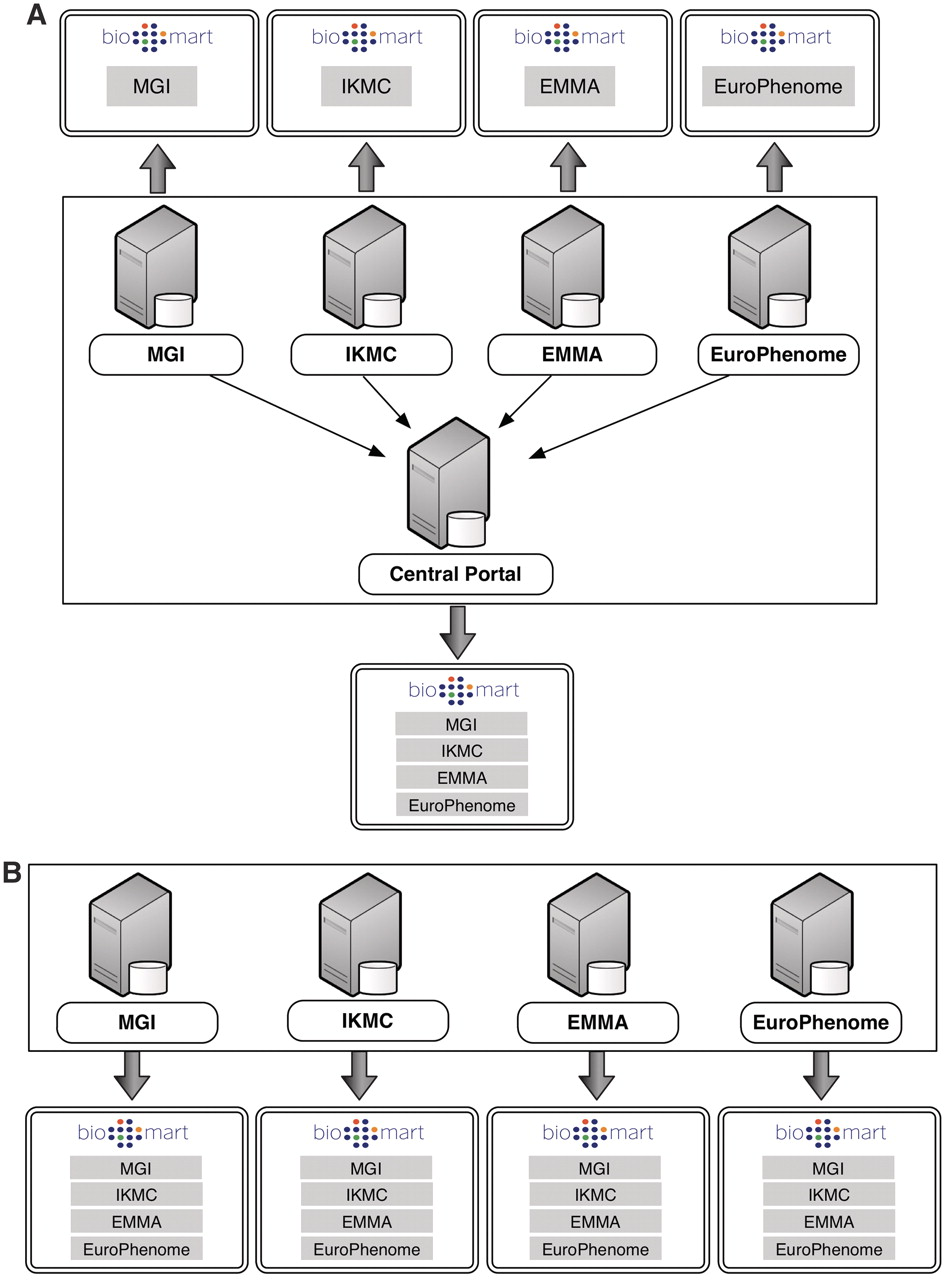
\includegraphics[width=\textwidth]{figures/biomart.png}
\caption[Biomart Portal Architecture.]{Biomart Portal Architecture. The portal can be set either with a master/slave or with a peer-to-peer configuration.
\label{fig:biomart}}
\end{figure}

Given the inclusion of a multi-database paradigm, the BioMart team developed a server that provide access to a collection of sources called a BioMart Portal. Figure \ref{fig:biomart} shows the 2 possible configurations of the BioMart Portal. In the configuration (a) each data source serves their own data and an independent server works as a central portal generating a unified view of the whole system. Alternatively, in the configuration (b) all the data source are treated as peers and they communicate with each other in order to be able to provide not only their own data, but also its peers' data.

BioMart includes a tool to automatically transform any 3rd form normalised database schema into the reverse-star scheme type used by this system. Once the dataset have been transformed, BioMart provides different view ports to it: Web-based Graphic Interface, Restful services and API connectors using Java.



\subsubsection{BioMOBY}
\subsubsection{Taverna and Galaxy}
\subsubsection{Bio2RDF}
\subsubsection{WikiGenes and WikiProteins}

\subsection{The Distributed Annotation System}
The Distributed Annotation System (DAS) is... \cite{JEN2008} and I can use Fig.~\ref{fig:das}. to explain:
\begin{figure}  
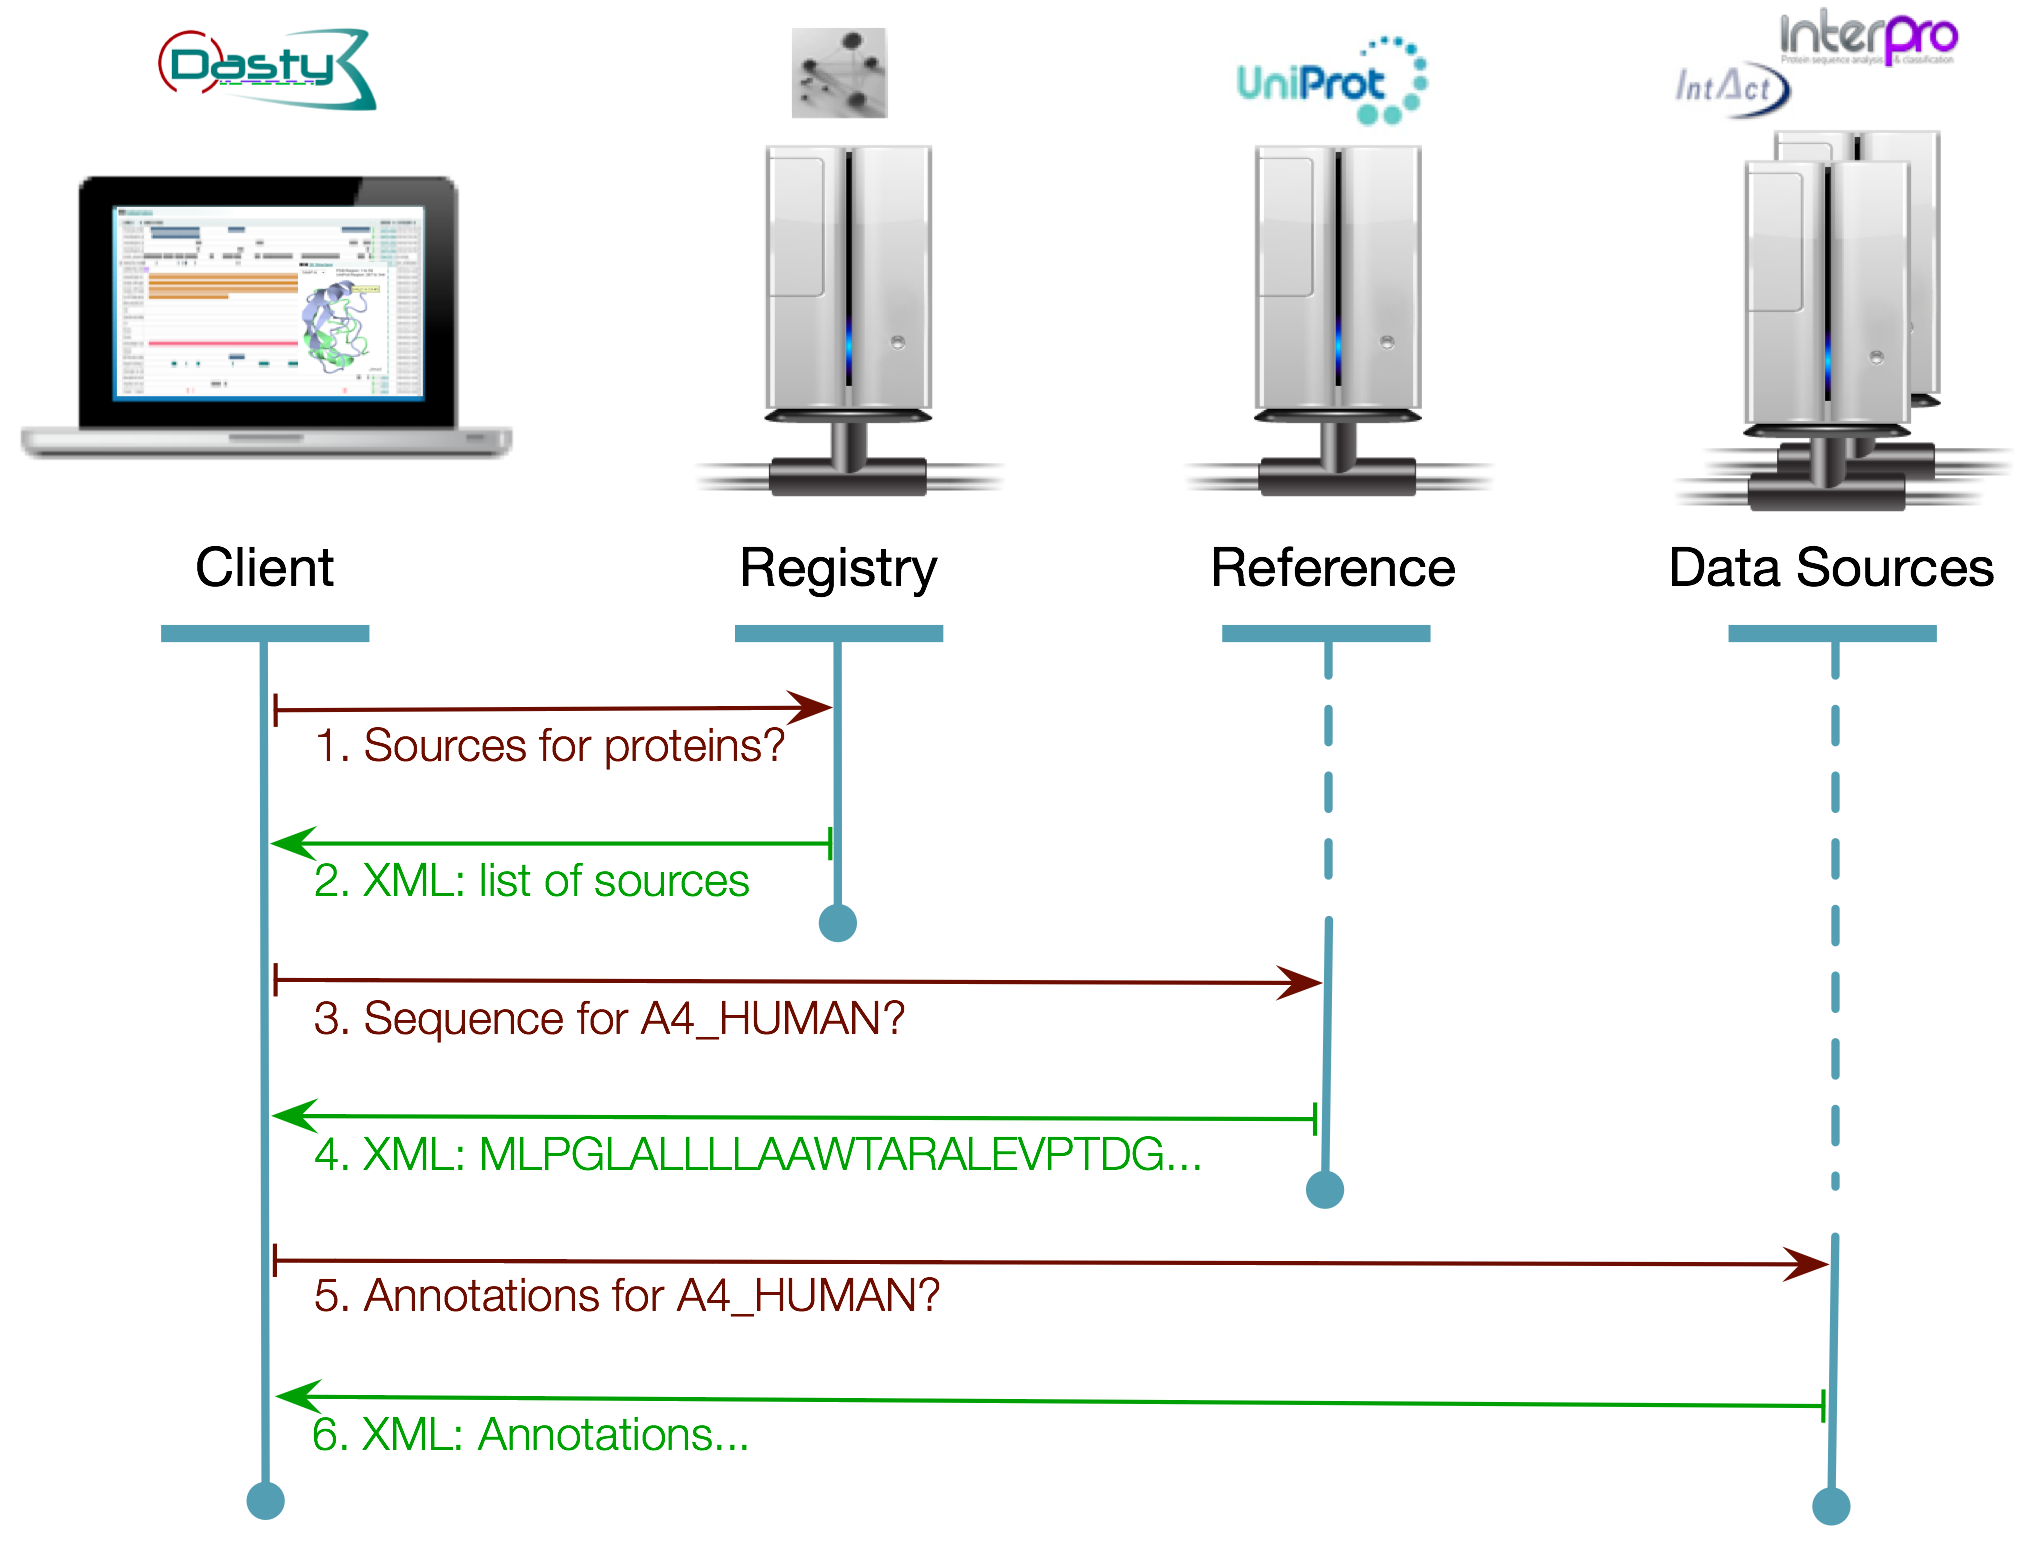
\includegraphics[width=\textwidth]{figures/DAS.png}
\caption[DAS Flow of Information.]{Flow of information in a standard query in the Distributed Annotating System.
\label{fig:das}}
\end{figure}
we should describe Dasty3 \cite{VIL2011}

\begin{savequote}[75mm] 
Our posturings, our imagined self-importance, the delusion that we have some privileged position in the Universe, are challenged by this point of pale light.
\qauthor{Carl Sagan, Pale Blue Dot, 1994} 
\end{savequote}
\section{Visualization}
The field of visualization aims to represent data in a way that non evident features became visible. The developed techniques in this search varies from simple ones (e.g. histograms) to very elaborated (e.g. environments just visible using 3D virtual reality rooms).

The uses of visualization techniques are as diverse as fields are in the world, from weather forecast in the news to the analysis of the captured data in the Large Hadron Collider. In the field of our interest: bioinformatics, the use of visualization methods is also abundant and sub-fields such as genomics, proteomics, population variance, etc. have plenty of examples were different techniques have been implemented with the purpose of making sense of biological data via visual representations.

The section below is a review of the most relevant existing tools in different bioinformatics fields.
\subsection{Visualization tools in Bioinformatics}
Small intro for the subsection
\subsubsection{Genomics}
Ensembl, mykarioView, Dalliance, IGV, Tablet, BAMView
\subsubsection{Proteomics}
Dasty, Interpro
\subsubsection{Protein Interaction}
\subsubsection{Population Variation}
\subsubsection{General Research}
To talk about statistical graphs and things like heat maps, phylogenetic trees, etc.


\section{Thesis outline}
